\documentclass[a4paper]{article}

\usepackage[british,UKenglish,USenglish,english,american]{babel}
\usepackage{inputenc}
\usepackage{url}
\usepackage{graphicx}
\usepackage{caption}
\usepackage{subcaption}

\begin{document}
\title{Summary}
\maketitle

\section{Intro}
Here, the results obtained in with frav data experiment of using imagenet are discussed.\\

\section{Architecture}
The architecture is like the imagenet one. Weights are not initilizad with a gaussian function. Also, it is used logistic regression as aclassifier.\\

\section{Database}
The database used is the frav one. In which there are 2398 trianing samples (119 batches), 342 validation samples (17 batch), 685 test samples(34 batches).\\

Faces are located using opencv, cropped and rescale into 5 different sizes. Each face of each scale is resize into 128x128 px and saved.\\

\begin{table}[]
\centering
\caption{My caption}
\label{my-label}
\begin{tabular}{lllll}
        & Training & Testing & Validation &  \\
Class 0 & 662      & 68      & 35         &  \\
Class 1 & 1736     & 617     & 307        &  \\
        &          &         &            & 
\end{tabular}
\end{table}


It is important to know that the difference between the number of samples in training, test and validation of class 0 and class 1 are really different. The proportion between classes in training is 2.5 times, in test 9times and in validation 8.7 times. This is because samples are read and pseudo-random shuffle and then distrubuted.\\


\section{Esperiment}
The experiment runs for 400 epoch with a learning rate of 0.001

\section{Results}
The best validation score of 1.470588 \% has been obtained at iteration 27965, with test performance 5.000000 \%

\begin{table}[]
\centering
\caption{My caption}
\label{my-label}
\begin{tabular}{lllll}
TP & TN  & FP & FN &  \\
61 & 609 & 3  & 7  &  \\
   &     &    &    &  \\
   &     &    &    & 
\end{tabular}
\end{table}

Class 0 (attacks) has been misclassified 7 times.\\
Class 1 (real users) has been misclassified 3 times.\\

\begin{figure}[htb]
\centering
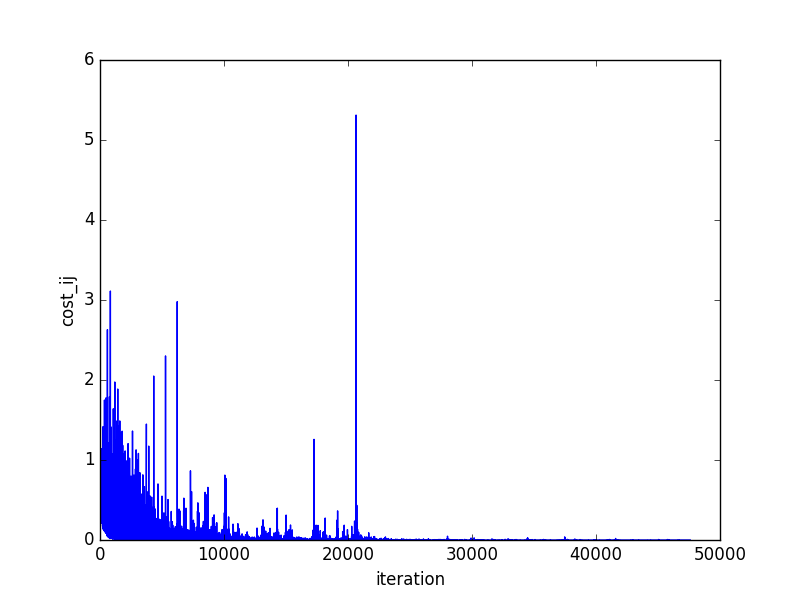
\includegraphics[width=0.45\textwidth]{images/cost_frav.png}
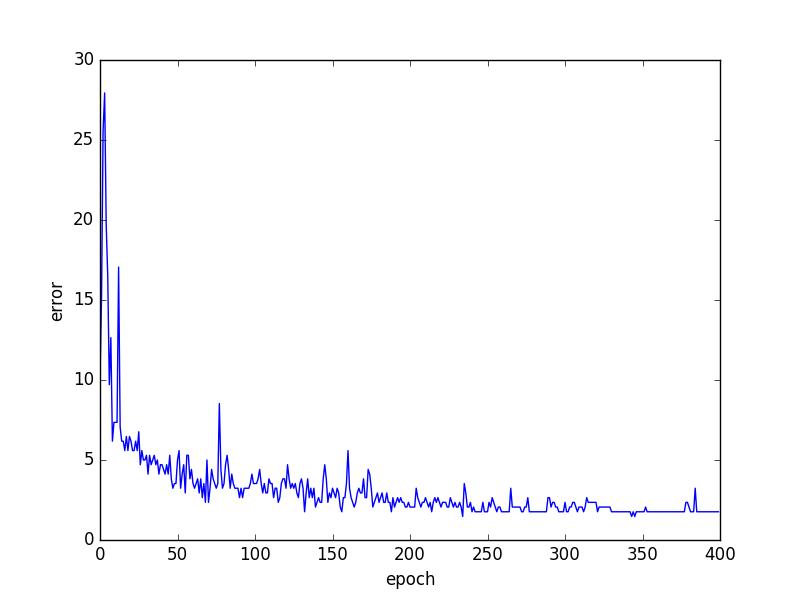
\includegraphics[width=0.45\textwidth]{images/error_frav.png}
\caption{Error rate and cost during the training} \label{fig:ErrorCost}
\end{figure}

In figure \ref{fig:ErrorCost}, The cost and error get stabilize in the last 200 epoch from 400 epoch. The error decreases its value from almost 30\% to 1.5\% which is a really low rate. When weights and biases are saved in the best validation iteration and loaded to test, a 5\% error rate has gotten. Which is a good result. Just 10 images has been misclassified. 7 images were faces from attacks and 3 images from users.

\begin{figure}[htb]
\centering
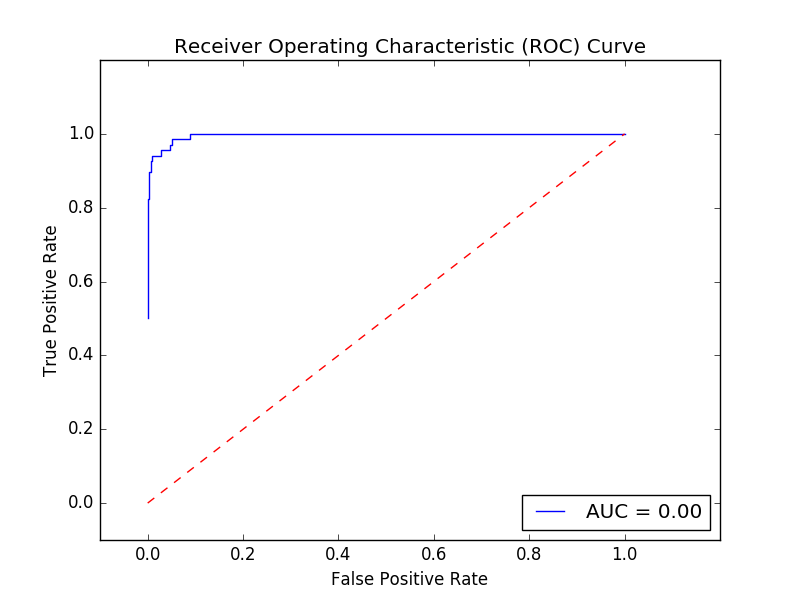
\includegraphics[width=0.45\textwidth]{images/ROC.png}
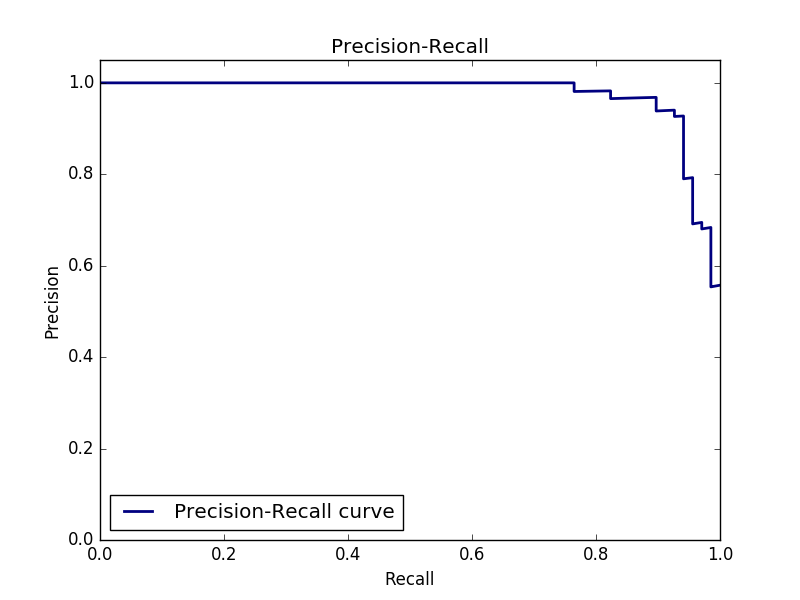
\includegraphics[width=0.45\textwidth]{images/Precision-Recall.png}

\caption{Error rate and cost during the training} \label{fig:ROCPrecisionRecall}
\end{figure}



\end{document}